\chapter{预备知识}\label{Guide}
本章详细说明本文研究所需要掌握的基础知识。第一节解释了多方安全计算问题的定义和需要满足的性质以及多方安全计算程序的执行过程。第二节较为完整的说明了Wys*的特性,实现安全计算的方法以及特殊结构的功能。第三节介绍了Wys*的电路编译过程并给出了Wys*语法中能够进行电路编译的语法子集。
\section{多方安全计算}
在一个SMPC定义中\citep{evans2017pragmatic},一组$n$个参与者$p_1,p_2,\dots,p_n$各自拥有隐私数据$d_1,$ $d_2,\dots,d_n$。参与者们在计算一个依赖于各方隐私数据的公开函数$f(d_1,d_2,\dots,d_n)$ 的同时保持各自输入的$d_i$的隐秘性。基于完全可信的第三方的解决方案十分朴素,由第三方$s$分别接受各个参与者的输入$d_i$,由$s$计算出$f(d_1,d_2,\dots,d_n)$的结果$z$后,返回$z$给各个参与者$p_i$。完全可信的第三方是不存在的,因此基于可信第三方的解决方案带来的问题是显而易见的。使用技术手段解决SMPC问题的途径有两种,一种是基于可信硬件(例如Intel SGX),另一种是基于密码学协议的多方安全计算协议(例如GMW协议,BMR协议等),本文介绍基于多方安全计算协议的多方安全计算。基于完全可信的第三方是最理想情况下的解决方案,在该方案下的计算过程中,每个参与者$p_i$得到的信息只有各自的输入$d_i$以及计算结果$z$,此外没有任何的额外信息能够用于推测其他参与者的输入。多方安全计算协议为了达到安全性至少需要满足两个属性:
\begin{itemize}
	\item 输入数据$d_i$的隐私性。计算过程中$p_i$获得的除$d_i$和$z$以外的任何中间数据对于推测其他参与者的输入没有任何帮助。
	\item 正确性。任何参与者的作弊行为或联合作弊行为都不能迫使诚实的参与方获得错误的结果$z$,这意味着计算结束时诚实的参与者一定能得到正确的结果,否则协议会在计算结束前中止。
\end{itemize}

多方安全计算协议发展至今,姚智期的混淆电路协议、GMW协议\citep{goldreich2019play}、BMR协议\citep{beaver1990round}等诸多协议在不同的安全假设下实现了多方安全计算,此外还出现了为特定的多方安全计算问题专门优化的协议,如解决隐私集合求交集问题的PSSZ协议\citep{pinkas2015phasing}等。我们将基于多方安全计算协议开发的用于解决多方安全问题的程序称为多方安全计算程序,目前已有许多用于开发多方安全计算程序的框架,如Sharemind、Wysteria、Obliv-C等\citep{bogdanov2008sharemind, rastogi2014wysteria, zahur2015obliv},这些框架整合了多方安全计算程序需要的网络和密码学程序库、多方安全计算协议实现、电路编译器、程序解释器等组件,提供了不同需求场景下的多方安全计算程序开发平台。

一个多方安全计算程序的执行包含许多过程,如图\ref{fig:smpc}。一般来说,当解释器解释执行一个多方安全计算程序时,本地计算内容在本地完成,多方计算函数先被编译为布尔电路或算术电路,然后作为多方安全计算协议的输入,主程序此时暂停执行,等待获得多方计算的结果后再继续执行。多方协议执行时通过网络与各方进行通信,等待各方协议执行完成进行同步再将结果返回给主程序。
\begin{figure}[!htbp]
    \centering
    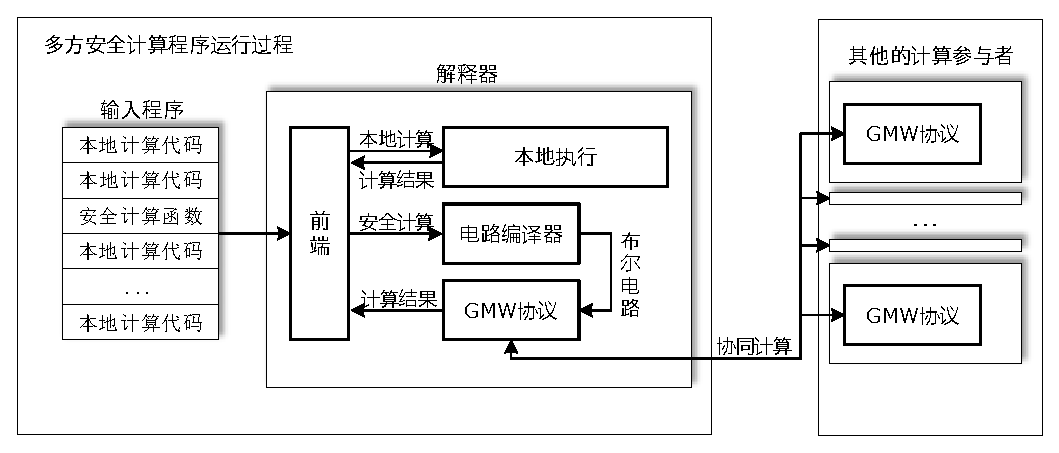
\includegraphics[width=1.00\textwidth]{SMPC.pdf}
    \caption{多方安全计算程序的执行过程}
    \label{fig:smpc}
\end{figure}

\section{Wys*:多方安全计算领域特定语言}
Wys*是Aseem Rastogi等人设计和开发的面向验证的多方安全计算的领域特定语言,Wys*的前身是同样用于开发多方安全计算程序的Wysteria\citep{rastogi2014wysteria}。Wys*底层使用拥有丰富验证功能的Fstar,在完成了前身Wysteria的功能同时完成了对自身的形式化验证。Wys*中利用联合类型声明了一类用于区分不同参与者标识的关键字Alice,Bob,Charlie等,这些标识除了区别参与者身份外,还被用于区别不同参与者来源的数据以及限制隐私数据的访问权限。 

Wys*有两个最重要的特点\citep{rastogi2019textsc}:
\begin{itemize}
	\item Wys*为SMPC设计了清晰的程序逻辑:Wys*的程序设计为混合模式,由本地计算,程序交互和安全计算三种模式组成。Wys*的程序模式使应用程序可以编写为与分布式语义等价的单线程语义的形式,解决了不同参与方各自拥有一份不同实现的情况。基于Fstar的验证能力,Wys*在程序中嵌入前置条件和后置条件来检查程序逻辑,并为检查用户指定的安全属性提供了可供观察的信息。
	\item Wys*实现了丰富的功能,其中一部分经过形式化验证。Wys*使用解释器在本地执行本地计算,安全计算函数先被解释器翻译为布尔电路,然后被一个基于GMW协议的库程序执行。Wys*还特别包含了一组外部函数接口用于利用Fstar的程序库。
\end{itemize}
在Wys*的整个实现当中,除了一个控制程序推进的函数、GMW协议程序、电路编译以及Fstar的工具链之外,其他部分都经过了形式化的验证,解释器正确性也经过了证明。 

除了保留Alice、Bob等参与者标识关键字外,Wys*在实现时引入了一系列安全计算的内容,\textbf{as\_par}和\textbf{as\_sec}是两种特定模式下计算的声明,\textbf{as\_par}有两个参数$ps$和$g$,$ps$是一组参与者标识的集合,$g$是一个待计算函数,解释器执行到\textbf{as\_par}时,$ps$中的参与者在本地执行$g$中的运算,计算的结果将被打上参与者的标签存储在本地用于后续运算,未包含在$ps$中的参与者则跳过该表达式。\textbf{as\_par}的目的是提供实现高效的多方安全计算程序,将隐私数据中不敏感或者不需要多方计算的部分拆分在本地执行,这样可以明显的提高程序效率。\textbf{as\_sec}是Wys*进行安全计算的核心,\textbf{as\_sec}同样有$ps$和$g$两个参数,当解释器执行到\textbf{as\_sec}时,解释器将函数$g$对应的语法树编译为布尔电路,然后调用GMW协议执行该电路,$ps$中声明的参与者通过GMW协议协同计算函数$g$的结果,并各自将结果存储在本地。Wys*在进行安全计算之前,隐私数据先被使用\textbf{box}表达式封装起来,\textbf{box}接受一组参与者集合$ps$和一组数据$v$,$v$被封装为只能被$ps$中的参与者访问和解封的封装类型,保证安全计算期间隐私数据不会被其他参与者访问。当需要进行计算时,再通过\textbf{unbox}表达式进行解封取出其中的值进行运算。 

当需要\textbf{as\_sec}向参与者返回不同的结果时,Wys*设计映射方法来完成,以百万富翁问题为例,$true$代表财富多于对方,那么两方的结果中必定一个为$true$另一个为$false$。\textbf{mkmap}表达式接受一个参与者集合参数$ps$和一个计算表达式$e$,创建一个从$ps$中的参与者到$e$的计算结果的映射;\textbf{project}表达式接受一个参与者$p$和一个映射$m$,从映射$m$中取出参与者$p$对应的值;\textbf{concat}表达式接受两个映射$m_1$、$m_2$,将两个映射合并后产生新的映射$m_0$。Wys*通过外部函数接口FFI(Foreign Function Interface)使用F*的本地函数,FFI $f$ $e$表达式调用F*的函数$f$并给予参数$e$,FFI中大部分列表运算需要的函数能被用于任何位置。FFI简化了Wys*的核心部分,使Wys*不会为了实现基础辅助函数功能变得臃肿,同时也避免了Wys*因此失去安全属性保证。



\section{Wys*的电路编译}\label{trans}
Wys*的电路翻译部分没有使用第三方程序而是使用了自己实现的电路编译模块,本文研究过程中假设Wys*的电路编译模块的正确性是可信的。整个编译过程分两大部分,第一部分将安全计算函数的语法树编译为逻辑电路,逻辑电路的组成元素包括二元运算符、自然数常量、布尔值常量、多选器、复制运算这些高级元素。第二部分将逻辑电路编译为完全由与门和异或门组成布尔电路。Wys*的电路编译能力有一定的限制,电路编译功能接受的输入是一个Wys*语法的子集。
\begin{equation*}
\begin{split}
\text{expression}\ e \coloneqq &\  x \\
\vert &\ c \\
\vert &\ \textbf{unbox}\ e \\
\vert &\  \textbf{let}\  x=e_1\ \textbf{in}\ e_2  \\
\vert &\  e_1\ op\ e_2 \\
\vert &\ \textbf{if}\ e_1 \ \textbf{then}\ e_2 \ \textbf{else}\ e_3 \\
\vert &\ ffi
\end{split}
\end{equation*}
这个子集是一系列表达式的集合,包括常数、变量、解封装、局部绑定、二元运算、条件分支和一类外部函数。外部函数中的函数可以在安全计算函数中使用,电路编译时这些函数会被Wys*表示成电路的形式。
\begin{equation*}
\begin{split}
\text{FFI}\ ffi \coloneqq &\  \textbf{FFI.mk\_nil} \\
\vert &\ \textbf{FFI.mk\_cons}\ e_1\ e_2 \\
\vert &\ \textbf{FFI.nth}\ e_1\ e_2 \\
\vert &\ \textbf{FFI.list\_mem}\ e_1\ e_2 \\
\vert &\ \textbf{FFI.list\_intersect}\ e_1\ e_2 
\end{split}
\end{equation*}
受限于Wys*的电路编译模块,逻辑电路只能接受两种布尔二元运算和两种算术二元运算。加法、减法、大于比较运算符的操作数必须是整数,等于比较运算符的操作数可以是布尔值、整数和整数列表。
\begin{equation*}
\begin{split}
\text{operator}\ op \coloneqq &\  \textbf{>}\ | \textbf{=}\ | \textbf{+}\ | \textbf{-} \\
\text{constant}\ c \coloneqq  &\ \textbf{true}\ | \textbf{false}\ | \text{integer constant} 
\end{split}
\end{equation*}
以上的语法描述了Wys*电路编译功能所接受的表达式类型的清晰面貌,但是它的编译能力还受到数据类型的限制:电路输入数据类型为布尔值、自然常数、整数列表以及封装类型;输出结果的类型为布尔值、自然常数以及整数列表;封装表达式\textbf{unbox}的参数类型必须是一个封装类型,而封装类型作用于布尔类型、自然常数以及整数列表;Wys*将安全计算函数按照上述规则编译为逻辑电路后,按照对应关系再将逻辑电路编译为布尔电路。基于Wys*电路编译模块功能正确性的假设,第一阶段的逻辑电路编译成功后,第二阶段的布尔电路编译过程必然成功,所以本文将注意力集中于逻辑电路编译过程,布尔电路编译不展开讨论。